\documentclass[runningheads]{llncs}

\usepackage[utf8]{inputenc}
\usepackage[numbers, comma, sort]{natbib}
\bibliographystyle{apalike}

\usepackage{amssymb}
\setcounter{tocdepth}{3}
\usepackage{graphicx}
\usepackage{float}

\usepackage{wrapfig}


\usepackage{pgfplots}
\usepackage{tikz}
\usetikzlibrary{arrows,backgrounds,positioning}
\usepackage{todonotes}

\usepackage{url}
\urldef{\mailsa}\path|rob@clabs.cc,schubotz@tu-berlin.de |
\newcommand{\todaydate}{\leadingzero{\day}.\leadingzero{\month}.\the\year}
\newcommand{\keywords}[1]{\par\addvspace\baselineskip
\noindent\keywordname\enspace\ignorespaces#1}

\begin{document}

\mainmatter

\title{Mathematical Language Processing \\ Project}
\titlerunning{MLP}

\author{Robert Pagel \and Moritz Schubotz}
\authorrunning{Pagel, Schubotz}

\institute{
Database Systems and Information Management Group,\\
Technische Universit\"{a}t Berlin,
Einsteinufer 17, 10587 Berlin, Germany\\
\mailsa\\
\url{http://demo.formulasearchengine.com/}}


\maketitle


\begin{abstract}

In natural language, words and phrases themselves imply the semantics. In contrast, the meaning of identifiers in mathematical formulae is undefined.
Thus scientists must study the context to decode the meaning. The \emph{Mathematical Language Processing} (MLP) project aims to support that process.  In this paper, we compare two approaches to discover identifier-definition tuples.  At first we use a simple pattern matching approach. Second, we present the \emph{MLP} approach that uses Part-of-speech (POS) tag based distances as well as sentence positions to calculate indentifier-definition probabilities. The evaluation of our prototypical system, applied on the Wikipedia text corpus, shows that our approach augments the user experience substantially. While hovering the identifiers in the formula, tool-tips with the most probable definitions occur. Tests with random samples show that the displayed definitions provide a good match with the actual meaning of the identifiers.


\keywords{definition discovery, text mining, parallel computing}
\end{abstract}


\section{Introduction}

\begin{wrapfigure}{r}{0.4\textwidth}
\label{fig:screenshot}
\vspace{-20pt}
	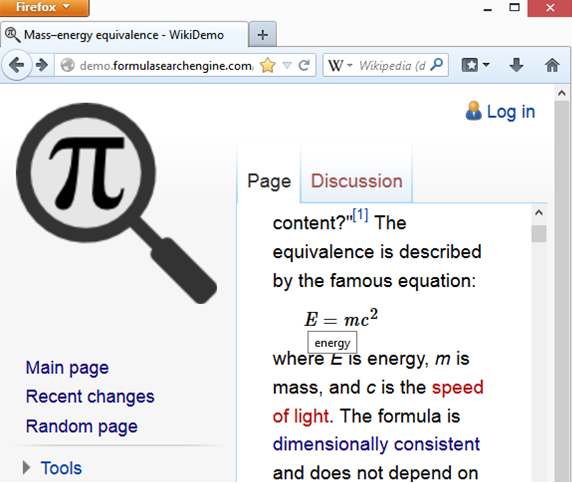
\includegraphics[width=0.4\textwidth]{screenshot}
\caption{Screenshot of the energy mass relation page `Mass–energy equivalence', while hovering the letter `E'.}
\vspace{-20pt}
\end{wrapfigure}

Mathematical formulae are a viable source of information for a wide range of
scientists. Often, they contain identifier whose meaning might be at first
unknown or at least ambiguous to the reader (depending on their knowledge).
Therefore, one usually needs to study the surrounding text to find the
relevant definition. An automatic information retrieval system can be used to
reduce the reader's effort by showing the most relevant definition relation
found to the reader. Students and scientists of other disciplines would
especially profit from a system that helps them to understand formulae more
quickly. In the long term the extracted identifier definition tuples contribute
to an increase of machine readability of scientific publications. This builds a 
foundation for added value services such as search, clustering and improved
accessibility.


To build such a system, a labelled text corpus that annotates identifiers and
their definition is desirable. At the project start, such a corpus was not
available. 
We assume that the probability to find correct identifier definition tuples is
POS tagged based distance metrics.
Our motivation for that is readers usually extract the identifier definition
from the context that is given by the surrounding text.
In combination with the Stratosphere system
that is capable of scalable data processing,  we rapidly generate a large
amount of definition relation candidates with only minimal implementation
overhead for the parallelization.


We chose the Wikipedia text corpus as a target because of two facts. First,
most articles make use of \texttt{<math/>} tags (\emph{texvc} as an input
language) for formulae. Those tags are easy to detect and the extraction identifiers
in its experimental MathML output format is well tried. 
Second, the text is already annotated with mark-up.
Particularly, hyperlinks to other articles within the Wikipedia are of
interest as they typically wrap around any number of words and indicate that
these in combination are relevant in the given context (respectively
sentence).


The English Wikipedia contains roughly four million articles. Even if we only
pick articles containing \texttt{<math/>} tags, our processor still needs to
compute with tens of thousands of articles. Especially when using text
annotators (e.g. \emph{POS} tagger \cite{Rathna96}), like Stanford's NLP
framework, one can make use of a parallel processing system to speed up
computation. Therefore we implement the proposed strategy with the
Stratosphere system based on the PACT programming model \cite{Alexandrov2010}.


\paragraph{Related Work.}

\citeauthor{Quoc2010} \cite{Quoc2010} proposed an approach for
relating whole formulas to sentences and their describing paragraphs.
\citeauthor{Yokoi} \cite{Yokoi} trained a \emph{support vector machine} to extract
natural language descriptions for mathematical expressions.

\section{Pattern-based Definition Discovery}

At first, we implemented a simple identifier definition extractor that is
based on a set of static patterns. As it is an fairly robust approach and easy
to implement, this will serve us as a good reference point in terms of
performance. The following patterns are being used to discover description
terms:

\begin{table}
\vspace{-5pt}
	\begin{center}
		\begin{tabular}{| p{9.3cm} |}
			\hline
			Pattern \\
			\hline
			\texttt{\emph{<description>} \emph{<identifier>}} \\
			\texttt{\emph{<identifier>} is \emph{<description>}} \\
			\texttt{\emph{<identifier>} is the \emph{<description>}} \\
			\texttt{let \emph{<identifier>} be the \emph{<description>}} \\
			\texttt{\emph{<description>} is|are denoted by \emph{<identifier>}} \\
			\texttt{\emph{<identifier>} denotes */DT \emph{<description>}} \\
			\hline
		\end{tabular}
	\end{center}
\caption{Implemented static patterns}
\vspace{-5pt}
\end{table}

Note that in the last pattern we used a \emph{part-of-speech} tag. Actually
determiners not only contain articles but also quantifiers and distributives.
To increase readability this list have been shortened to `*/DT'.
\todo[inline]{describe the process: extraction of identifiers, how to didentify the dscription? Looking for space or using pos tags?}


\section{Statistical Definition Discovery}

We detect relations between identifiers and their description in two steps.
First, we extract the identifiers from the formulae found in an article and
second we determine their description from the surrounding text.

Extracting relevant identifiers from the article rely on the assumption that
the author will use \texttt{<math/>} tags for all formulae. This said, a
formula that is written within a text cannot be recognized, and therefor, any
identifier that is solely used there, can never be extracted.

The fact that we can estimate all relevant identifiers for an article (see
Section \ref{ir}), combined with some common assumptions about the relation,
can be exploited to largely reduce the set of candidates that need to be ranked.
Please note that this reduction is essential for retrieving the correct
relations. Otherwise almost any word would be ranked and the precision of the
retrieval would drop significantly.

The basic assumption of outr approach is that the two entities of a definition
relation co-occur in the same sentence.

The basic assumption of our approach is that if two entities take part in a
relation, those two co-occur in the same sentence.
Any other sentence is, therefor, irrelevant.

Another assumption can be made about the lexical class
of the desciption we want to rank. They are nouns or even noun phrases (e.g.
\texttt{ `the effective spring constant k' } or \texttt{ `mass m of
something'} ). Beside discarding all other words (according to their POS tag),
noun phrases and terms within a Wikipedia hyperlink will be aggregated into
one new candidate term. This is important, due to the fact that overall
ranking will be greatly infuenced by the distance of candidate words. For all
intends and purposes, it is not needed to keep noun phrases as single words.
So they can be aggregated and be ranked as if they were a single word.


\subsection{Numerical Statistics}

Each description candidate is ranked with the weighted sum

\begin{equation} \label{eq:rating}
R(n,\Delta,t,d)=\frac{\alpha{R}_{\sigma_\mathrm d}(\Delta)
+\beta{R}_{\sigma_\mathrm s}(n)
+\gamma\mathrm{tf}(t,s)}{\alpha+\beta+\gamma} \mapsto [0;1].
\end{equation}

It depends on the distance $\Delta$ (= amount of word tokens) between
identifier and the description term $t$, the sentence number $n$ counting
(from the beginning of the article) all sentences containing the identifier,
and the term frequency $\mathrm{tf}(t,s)$ in the set of sentences $s$. The
distance was normalized with $R_\sigma(\Delta) = \exp\left[ -\frac{1}{2}
\frac{\Delta^2-1}{\sigma^2}\right].$ We assume that the probability to find a
relation at $\Delta=1$ is maximal. For example in the text fragment
\texttt{`the energy E, and the mass m'}, in order to determine the full width
at half maximum of our distribution, we evaluated some articles manually and
found $R_{\sigma_\mathrm d}(1)\approx 2 R_{\sigma_\mathrm d}(5)$ and thus
$\sigma_d=\sqrt\frac{12}{\ln 2}$. The probability to find a correct definition
decays for 50\% within three sentences. Consequently $\sigma_\mathrm
s=2\left({\ln 2}\right)^{-\frac{1}{2}}$.


\paragraph{Robustness.}

The classic tf-idf \cite{Salton86} statistic reflects the importance of a term
to a document. For our task, the inverse document frequency (idf) would assign
high penalties to frequent words like `length', in comparison to words seldom
seen like `Hamiltonian', which are both valid definitions for identifiers. As the
influence of $\mathrm{tf}(t,s)$ on the sensivity of the overall ranking
(\ref{eq:rating}) seems to be very high, we reduce the impact with the tuning
parameters $\gamma=0.1$ and $\alpha = \beta = 1$. Please note that this work
is still in progress. For now the algorithm only takes the sentences into
account, that were found in a single article. In the future, the retrieval
process will take sets of closely related articles into account, trying
leverage the problem that distributional properties will be volatile on term
universes with very few members (e.g. term frequencies in a single sentence).


\paragraph{Implementation.}

We implemented the MLP processing system \cite{github} as Stratosphere data-
flow using Java which allows for scalable execution, application of complex
higher order functions and easy integration of third party tools like Stanford
NLP and the Mylyn framework for mark-up parsing.


\tikzset{actor/.style={
        rectangle,
        minimum size=6mm,
        very thick,
        draw=gray!50!black!50,
        top color=white,
        bottom color=gray!50!black!20
    },
    arrow/.style={
        -latex, thick, shorten <=2pt,shorten >=2pt
    }
}
\begin{figure}[H]
	\begin{tikzpicture}[node distance=5mm and 8mm]
		\node (Input) [align=center]{Wiki Dumps};
		\node (DocumentParser) [actor, right=of Input, align=center] {\emph{Map}\\\textbf{Parser}};
		\node (Candidates) [actor, right=of DocumentParser, align=center] {\emph{CoGroup}\\\textbf{Kernel}};
		\node (Sentence) [actor, above=of DocumentParser, align=center] {\emph{Map}\\\textbf{Tagger}};
		\node (Filter) [actor, right=of Candidates, align=center] {\emph{Reduce}\\\textbf{Filter}};
		\node (Output) [right=of Filter,align=center]{Raw\ Candidates};
		\draw[arrow] (Input)--(DocumentParser);
		\draw[arrow] (DocumentParser)--(Sentence);
		\draw[arrow] (DocumentParser)--(Candidates);
		\draw[arrow] (Sentence.east)--(Candidates.north);
		\draw[arrow] (Candidates)--(Filter);
		\draw[arrow] (Filter)--(Output);
	\end{tikzpicture}
\caption{Data flow of the Stratosphere program}
\end{figure}



\section{Evaluation}

\subsection{Identifier Retrieval}
\label{ir}

Throughout our experiments we made some observations that had an impact on the
accuracy of retrieving the correct set of indentifer. First of all, people
tend to incorrectly use \emph{texvc} trying to create formulas. E.g.,
\texttt{\textbackslash text\{log\}} is more often used than the correct
operator \texttt{\textbackslash log}. Another problem is that sometimes people
use indices as a form of `in field' annotation, like $T_{before}$ and
$T_{after}$. The identifier $T$ is defined in the surrounding text, but
neither $T_{before}$ nor $T_{after}$. There are more ambiguities. For example
the superscripted 2 in $x^{2}$ and $\sigma^{2}$ can be interpreted as the
power or as a part of the identifier. Another ambiguity is that the
multiplication sign can be omitted, so that it is undecidable for a naive
program whether $ab^{2}$ contains one or two identifiers.

We took a very conservative approach and preprocessed all formulas.
\texttt{\textbackslash text\{\}} blocks along with subscriptions containing
more than a single character will be removed before analysis. Superscripts
will also be ignored in terms of being a part of the identifier. Moreover, we
created a comprehensive blacklist to improve the results further. Short words
like `a' and `i', which are very common in the English language, could be
easily matched by our processor in the surrounding text if a formula contains
one of those identifier, and therefore, will also be blacklisted. Additionally,
we blacklist common mathematical operators, constants, and functions.

Because of the fact, that we do not have any annotated test corpora,
evaluation has to be performed by hand. Therefore, we took a sample of 30
random articles and counted all matches. The resulting estimates for the
identifier retrieval performance are: \emph{Recall: 0.99} and \emph{Precision:
0.86}, which satisfy our information needs, as we are mostly interested in recall
a this stage.


\subsection{Description Retrieval}
We ran the program on a dataset of about 20.000 articles, all containing
\texttt{<math/>} tags, and retrieved about 550.000 candidate relations. The
most common definition relations were:


\begin{table}[H]
	\begin{center}
	\begin{tabular}{| l | p{6.8cm} | l |}
		\hline
		Identifier & Descriptions & Count\\
		\hline
		$n$ & number & 1709 \\
		$t$ & time & 1480 \\
		$M$ & mass & 1042 \\
		$r$ & radius & 752 \\
		$T$ & temperature & 666 \\
		$\theta$ & angle & 639 \\
		$G$ & group & 635 \\
		\hline
	\end{tabular}
	\end{center}
\caption{Most common definition relations}
\end{table}


\paragraph{Observations.} We observed some poorly ranked relations. For
example, in the fragment \texttt{`where $\phi$ ( $r_{i}$ ) is the electrostatic
potential'} the distance
$\Delta(\phi, \mathsf{electrostatic\:potential} ) = 6$. This is due
to counting brackets and function arguments as words. Also wrongly tagged
words like `Hamiltonian' as an adjective leads to false negatives. Latter


\subsubsection{Comparative Evaluation}

Due to the lack of gold standard evaluation datasets to measure the
performance of identifer definition extractors, we've created on on our own.
This is a very time consuming job. At the moment the dataset only contains two
large articles (revision ids are included) with around 100 identifier
definitions. This dataset is also available on the project repository.


As in lots of articles, the ones in the evaluation dataset contain identifiers
whose description cannot be retrieved. This is due to two reasons. First and
foremost, the identifier found in a formula is never mentioned in the
surrounding text, and therefor, no description can be extracted. Second, the
identifier is somehow ambigious (see section~\ref{ir}) and has been dropped. Most
notably, identifiers like $I_{xx}$ will be discarded because of an ambigious
index that contains multiple letters.


Unfortunately 32 out of 99 identifiers from our dataset fall into that category.
We've decided to evaluate the performance of the remainder, as those 32 do not
convey any conceptual flaws. From the users standpoint, the overall performance
(in terms of recall) of such a system whould be rather annoying. As we are only
interested in evaluating the performance of the \emph{MLP Ranking} algoritm itself,
it is save to ignore those 32 identifers.

\begin{table}[H]
\vspace{-5pt}
	\begin{center}
		\begin{tabular}{| l | l | l | l |}
			\hline
			 & MLP-Ranking ($k=1$) & MLP-Ranking ($k=2$) & Pattern Matching \\
			\hline
			Precision &  0.872  &  0.915  &  0.911  \\
			Recall    &  0.839  &  0.892  &  0.733  \\
			\hline
		\end{tabular}
	\end{center}
\caption{Evaluation results. Note: $k$ equals the amount of the top ranked candidate definitions.}
\vspace{-20pt}
\end{table}

The results show that the unoptimized MLP approach keeps up with the
performance of the simple pattern matcher. Furthermore, we observed that it is
more robust in terms of recall, as it is less vulnerable to small changes in
the sentence structure.


\section{Further work}

Our original intuition was to discover grammatical patterns like
\texttt{`\emph{<identifier>} indicates/stands for/denotes
\emph{<description>}'} based on the statistical findings. However, our
impression is that this would not lead to significant performance gain.

The distance measure $R_{\sigma_d}$ fails for the example of
Fig.~\ref{fig:screenshot} since $\Delta(\mathsf{energy},E) =
\Delta(\mathsf{mass},m) = 2$. Unfortunately, one cannot simply detect
punctuation marks and introduce some kind of directed associativity (e.g.
inflicting a penalty on the ranking if the candidate relations spans over a
comma). That would lead to whole classes of relation `types' (in terms of the
grammatical structure) never being retrieved. We plan to mitigate this problem
by taking more closely related scientific articles (based on their specific
fields) into consideration and count the frequencies of the candidate
relations. The intuition behind this is, that articles of the same scientific
field will likely use the same definition for the identifiers. Moreover,
we hope to also mitigate the problem of `dangling' identifiers (those not
mentioned in the article itself), as their may be description in related
articles.


Currently, we use the ranking $R$ to identify the most probable description-
identifier tuple on each article, even if it occurs multiple times on the page.
For example, in the `Mass-energy equivalence' article, 21 sentences contain the
combination of the identifier $E$ and the noun `energy'. A promising approach,
is to use $R^\Sigma=\sum_{i=1}^n 2^{-i} R_i,$ where $R_i$ is a sorted list,
were $R_1$ is the highest ranked definition for that relation according to the
current measure $R$.


Furthermore, a systematic approach for determining a wise choice of the
ranking parameters should significantly improve the overall performance of our
system.


\section{Conclusion}

Our experiments showed that selecting candidates according to their POS tags
combined with numerical statistics about the text surface, can lead to quality
results. However, this approach is only applicable under certain conditions.
For identifiers which are seldom seen, our statistical approach tends to fail.
In that situation, other methods, especially supervised ones, are used to
bootstrap a language model. Unfortunately, they require a labeled test corpus
to measure the performance of a classifier that could be trained with our
generated data. Currently, we are planning to use the NTCIR-Math-10 Task, Math
Understanding Subtask gold standard dataset \cite{overview} for a comparable
evaluation.

During this project we had the impression that one could discover `namespaces'
(sets of documents, that use the same definitions for identifier) to aid in
the retrieval procress. Robert Pagel currently works in his diploma thesis on
this topic.


\paragraph*{Acknowledgments.}

Thanks to Howard Cohl for proof reading the paper and to Holmer Hemsen, the
course instructor of the database project course at TU-Berlin in Fall 2012.
The implementation and a first draft of this paper was completed in the
duration of this course.


\begingroup
\let\clearpage\relax
\bibliography{mlp-papers}
\endgroup

\end{document}

